%%%%%%%%%%%%%%%%%%%%%%%% INICIO QUADRO 01 - VOL 1 %%%%%%%%%%%%%%%%%%%%%%%%%%%%%%%
\begin{table}[!ht]
  \centering
  \renewcommand{\tablename}{Quadro}
  \caption{Rudimentos de Teoria}
  \label{Quadro_01}
  \begin{tabular}[t]{|l|l|l|}
    \hline

    %%% PRÓXIMA LINHA
    \multicolumn{3}{|l|}{\letraquadrada{A}}

    %%% PRÓXIMA LINHA
    \\
    \quadtitulo{Cavaquinho}
    &
    \quadtitulo{Violão Tenor}
    &
    \quadtitulo{Baixo}

    \\
    \quadtitulo{Bandolim} & \quadtitulo{Violão} & \em

    \\
    \quadtitulo{Viola} & \em & \em
    

    %%% PRÓXIMA LINHA
    \\
    \begin[fragment]{lilypond}
      \transpose c c { 
        \keepWithTag #'cv
        \include "claves.ly" 
      }
    \end{lilypond}
    &
    \begin[fragment]{lilypond}
      \transpose c c { 
        \keepWithTag #'vi
        \include "claves.ly" 
      }
    \end{lilypond}
    &
    \begin[fragment]{lilypond}
      \transpose c c { 
        \keepWithTag #'bx
        \include "claves.ly" 
      }
    \end{lilypond}

    \\
  \end{tabular}


  %%% PRÓXIMA LINHA
  \begin{tabular}[t]{|l|l|}
    \hline
    \letraquadrada{B} \quadtitulo{Compasso}
    & 
    \letraquadrada{C} \quadtitulo{Barra de Compasso}


    %%% PRÓXIMA LINHA
    \\
    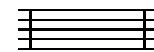
\includegraphics[scale=1]{compasso-vazio}
    &
    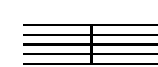
\includegraphics[scale=1]{barra-compasso}


    %%% PRÓXIMA LINHA
    \\
    \hline
    \letraquadrada{D} \quadtitulo{Compasso Quaternário}
    &    
    \letraquadrada{E} \quadtitulo{Barra Final}


    %%% PRÓXIMA LINHA
    \\
    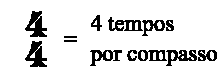
\includegraphics[scale=1]{formula-4tempos-por-compasso}
    &
    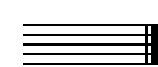
\includegraphics[scale=1]{barra-final}


    %%% FINAL DAS LINHAS
  \\
  \hline
  \end{tabular}
\end{table}    


%%%%%%%%%%%%%%%%%%%%%%%% FINAL QUADRO 01 - VOL 1 %%%%%%%%%%%%%%%%%%%%%%%%%%%%%%%

%%% complemento do QUADRO 01
\begin{center}
%#exemplo-01#%
\end{center}


%%%%%%%%%%%%%%%%%%%%%%%% INICIO QUADRO 02 - VOL 1 %%%%%%%%%%%%%%%%%%%%%%%%%%%%%%%
\begin{table}[!ht]
  \centering
  \renewcommand{\tablename}{Quadro}
  \caption{Cordas Soltas}
  \label{Quadro_02}
  \begin{tabular}[t]{|lll|}
    \hline


    %%% PRÓXIMA LINHA
    \letraquadrada{A} & \em & \em
   

    %%% CAVAQUINHO %%%%%%%%%%%%%%%%%%%%%%%%%%%%
    %%% PRÓXIMA LINHA
    \\
    \quadtitulo{Cavaquinho}    &\em    &\em


    %%% PRÓXIMA LINHA
    \\
    \quadtitulo
    &
    \quadtitulo
    &
    \quadtitulo


    %%% PRÓXIMA LINHA
    \\
    \begin[fragment]{lilypond}
      \transpose c c {
        \keepWithTag #'cv
        \include "nota-01.ly"
      }
    \end{lilypond}
    &
    \begin[fragment]{lilypond}
      \transpose c c { 
        \keepWithTag #'cv
        \include "nota-02.ly" 
      }
    \end{lilypond}
    &
    \begin[fragment]{lilypond}
      \transpose c c { 
        \keepWithTag #'cv
        \include "nota-03.ly" 
      }
    \end{lilypond}

    %%% BANDOLIM %%%%%%%%%%%%%%%%%%%%%%%%%%%%
    %%% PRÓXIMA LINHA
    \\
    \hline
    \quadtitulo{Bandolim}    &\em    &\em


    %%% PRÓXIMA LINHA
    \\
    \quadtitulo
    &
    \quadtitulo
    &
    \quadtitulo


    %%% PRÓXIMA LINHA
    \\
    \begin[fragment]{lilypond}
      \transpose c c {
        \keepWithTag #'bd
        \include "nota-01.ly"
      }
    \end{lilypond}
    &
    \begin[fragment]{lilypond}
      \transpose c c { 
        \keepWithTag #'bd
        \include "nota-02.ly" 
      }
    \end{lilypond}
    &
    \begin[fragment]{lilypond}
      \transpose c c { 
        \keepWithTag #'bd
        \include "nota-03.ly" 
      }
    \end{lilypond}

    %%% VIOLA %%%%%%%%%%%%%%%%%%%%%%%%%%%%
    %%% PRÓXIMA LINHA
    \\
    \hline
    \quadtitulo{Viola}    &\em    &\em


    %%% PRÓXIMA LINHA
    \\
    \quadtitulo
    &
    \quadtitulo
    &
    \quadtitulo


    %%% PRÓXIMA LINHA
    \\
    \begin[fragment]{lilypond}
      \transpose c c {
        \keepWithTag #'va
        \include "nota-01.ly"
      }
    \end{lilypond}
    &
    \begin[fragment]{lilypond}
      \transpose c c { 
        \keepWithTag #'va
        \include "nota-02.ly" 
      }
    \end{lilypond}
    &
    \begin[fragment]{lilypond}
      \transpose c c { 
        \keepWithTag #'va
        \include "nota-03.ly" 
      }
    \end{lilypond}

    %%% VIOLÃO TENOR %%%%%%%%%%%%%%%%%%%%%%%%%%%%
    %%% PRÓXIMA LINHA
    \\
    \hline
    \quadtitulo{Violão Tenor}    &\em    &\em


    %%% PRÓXIMA LINHA
    \\
    \quadtitulo
    &
    \quadtitulo
    &
    \quadtitulo


    %%% PRÓXIMA LINHA
    \\
    \begin[fragment]{lilypond}
      \transpose c c {
        \keepWithTag #'vt
        \include "nota-01.ly"
      }
    \end{lilypond}
    &
    \begin[fragment]{lilypond}
      \transpose c c { 
        \keepWithTag #'vt
        \include "nota-02.ly" 
      }
    \end{lilypond}
    &
    \begin[fragment]{lilypond}
      \transpose c c { 
        \keepWithTag #'vt
        \include "nota-03.ly" 
      }
    \end{lilypond}

    %%% VIOLÃO %%%%%%%%%%%%%%%%%%%%%%%%%%%%
    %%% PRÓXIMA LINHA
    \\
    \hline
    \quadtitulo{Violão}    &\em    &\em


    %%% PRÓXIMA LINHA
    \\
    \quadtitulo
    &
    \quadtitulo
    &
    \quadtitulo


    %%% PRÓXIMA LINHA
    \\
    \begin[fragment]{lilypond}
      \transpose c c {
        \keepWithTag #'vi
        \include "nota-01.ly"
      }
    \end{lilypond}
    &
    \begin[fragment]{lilypond}
      \transpose c c { 
        \keepWithTag #'vi
        \include "nota-02.ly" 
      }
    \end{lilypond}
    &
    \begin[fragment]{lilypond}
      \transpose c c { 
        \keepWithTag #'vi
        \include "nota-03.ly" 
      }
    \end{lilypond}

    %%% BAIXO %%%%%%%%%%%%%%%%%%%%%%%%%%%%
    %%% PRÓXIMA LINHA
    \\
    \hline
    \quadtitulo{Baixo}    &\em    &\em


    %%% PRÓXIMA LINHA
    \\
    \quadtitulo
    &
    \quadtitulo
    &
    \quadtitulo


    %%% PRÓXIMA LINHA
    \\
    \begin[fragment]{lilypond}
      \transpose c c {
        \keepWithTag #'bx
        \include "nota-01.ly"
      }
    \end{lilypond}
    &
    \begin[fragment]{lilypond}
      \transpose c c { 
        \keepWithTag #'bx
        \include "nota-02.ly" 
      }
    \end{lilypond}
    &
    \begin[fragment]{lilypond}
      \transpose c c { 
        \keepWithTag #'bx
        \include "nota-03.ly" 
      }
    \end{lilypond}

    \\
    \hline
  \end{tabular}
\end{table}


%%%%%%%%%%%%%% CONTINUAÇÃO DA TABELA
\begin{table}[!ht]
  \centering
  \begin{tabular}[t]{|l|l|l|}
    \hline

    %%% PRÓXIMA LINHA
    \letraquadrada{B}  & \letraquadrada{C}   &   \letraquadrada{D}
    
    %%% PRÓXIMA LINHA
    \\
    \quadtitulo{Mínima}
    &
    \quadtitulo{Semínima}
    &
    \quadtitulo{Técnica}


    %%% PRÓXIMA LINHA
    \\
    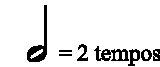
\includegraphics[scale=1]{minima}
    &
    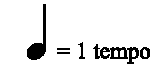
\includegraphics[scale=1]{seminima}
    &
    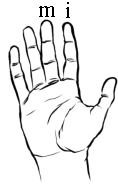
\includegraphics[scale=0.7]{mao-i-m}


    %%% PRÓXIMA LINHA
    \\
    \hline
    \letraquadrada{E}  & \letraquadrada{F} &   \letraquadrada{G}

    %%% PRÓXIMA LINHA
    \\
    \quadtitulo{Pausa de semibreve}
    &
    \quadtitulo{Pausa de mínima}
    &
    \quadtitulo{Sinal de Repetição}
    


    %%% PRÓXIMA LINHA
    \\
    
\includegraphics[scale=1]{semibreve-pausa}
    &
    
\includegraphics[scale=1]{minima-pausa}
    &
    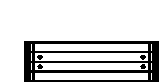
\includegraphics[scale=1]{sinal-repeticao}


    %%% FINAL DAS LINHAS
    \\
    \hline
  \end{tabular}
\end{table}    

%%%%%%%%%%%%%%%%%%%%%%%% FINAL QUADRO 02 - VOL 1 %%%%%%%%%%%%%%%%%%%%%%%%%%%%%%%%


%%%%%%%%%%%%%%%%%%%%%%%% INICIO QUADRO 03 - VOL 1 %%%%%%%%%%%%%%%%%%%%%%%%%%%%%%%
\begin{table}[!ht]
  \centering
  \renewcommand{\tablename}{Quadro}
  \caption{Sol Maior}
  \label{Quadro_03}
  \begin{tabular}[t]{|ll|ll|}
    \hline


    %%% PRÓXIMA LINHA
    \multicolumn{4}{|l|}{\letraquadrada{A}}
   
    %%% PRÓXIMA LINHA
    \\
    \multicolumn{2}{|l|}{\quadtitulo{Cavaquinho}} &    \multicolumn{2}{l|}{\quadtitulo{Bandolim}} 

    %%% PRÓXIMA LINHA
    \\
    \quadtitulo
    &
    \quadtitulo
    &
    \quadtitulo
    &
    \quadtitulo


    %%% PRÓXIMA LINHA
    \\
    \begin[fragment]{lilypond}
      \transpose c c {
        \keepWithTag #'cv
        \include "nota-04.ly"
      }
    \end{lilypond}
    &
    \begin[fragment]{lilypond}
      \transpose c c {
        \keepWithTag #'cv
        \include "nota-05.ly"
      }
    \end{lilypond}
    &
    \begin[fragment]{lilypond}
      \transpose c c {
        \keepWithTag #'bd
        \include "nota-04.ly"
      }
    \end{lilypond}
    &
    \begin[fragment]{lilypond}
      \transpose c c {
        \keepWithTag #'bd
        \include "nota-05.ly"
      }
    \end{lilypond}


    %%% PRÓXIMA LINHA
    \\
    \hline
    \multicolumn{2}{|l|}{\quadtitulo{Viola}} &    \multicolumn{2}{l|}{\quadtitulo{Violão Tenor}} 

    %%% PRÓXIMA LINHA
    \\
    \quadtitulo
    &
    \quadtitulo
    &
    \quadtitulo
    &
    \quadtitulo


    %%% PRÓXIMA LINHA
    \\
    \begin[fragment]{lilypond}
      \transpose c c {
        \keepWithTag #'va
        \include "nota-04.ly"
      }
    \end{lilypond}
    &
    \begin[fragment]{lilypond}
      \transpose c c {
        \keepWithTag #'va
        \include "nota-05.ly"
      }
    \end{lilypond}
    &
    \begin[fragment]{lilypond}
      \transpose c c {
        \keepWithTag #'vt
        \include "nota-04.ly"
      }
    \end{lilypond}
    &
    \begin[fragment]{lilypond}
      \transpose c c {
        \keepWithTag #'vt
        \include "nota-05.ly"
      }
    \end{lilypond}


    %%% PRÓXIMA LINHA
    \\
    \hline
    \multicolumn{2}{|l|}{\quadtitulo{Violão}} &    \multicolumn{2}{l|}{\quadtitulo{Baixo}} 

    %%% PRÓXIMA LINHA
    \\
    \quadtitulo
    &
    \quadtitulo
    &
    \quadtitulo
    &
    \quadtitulo


    %%% PRÓXIMA LINHA
    \\
    \begin[fragment]{lilypond}
      \transpose c c {
        \keepWithTag #'vi
        \include "nota-04.ly"
      }
    \end{lilypond}
    &
    \begin[fragment]{lilypond}
      \transpose c c {
        \keepWithTag #'vi
        \include "nota-05.ly"
      }
    \end{lilypond}
    &
    \begin[fragment]{lilypond}
      \transpose c c {
        \keepWithTag #'bx
        \include "nota-04.ly"
      }
    \end{lilypond}
    &
    \begin[fragment]{lilypond}
      \transpose c c {
        \keepWithTag #'bx
        \include "nota-05.ly"
      }
    \end{lilypond}

    \\
    \hline
  \end{tabular}

  \begin{tabular}[t]{|l|l|l|}

    %%% PRÓXIMA LINHA
    \letraquadrada{B} & \letraquadrada{C} & \letraquadrada{D}

    %%% PRÓXIMA LINHA
    \\
    \quadtitulo{Sol Maior}
    &
    \quadtitulo{Andamento}
    &
    \quadtitulo{Pausa de Semínima}

    %%% PRÓXIMA LINHA
    \\
    \begin[fragment]{lilypond}
      \transpose c c {
        \keepWithTag #'cv
        \include "armadura-sol.ly"
      }
    \end{lilypond}
    &
    \textit{Allegro}
    &
    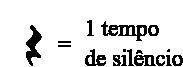
\includegraphics[scale=1]{seminima-pausa}



    %%% PRÓXIMA LINHA
    \\
    \hline
    \multicolumn{2}{|l|}{\letraquadrada{E}} & \letraquadrada{F}

    %%% PRÓXIMA LINHA
    \\
    \multicolumn{2}{|l|}{\quadtitulo{Fórmula de Compasso}}
    &
    \quadtitulo{Da Capo ao Fine}


    %%% PRÓXIMA LINHA
    \\
    \multicolumn{2}{|l|}{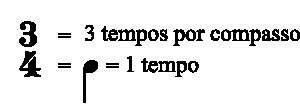
\includegraphics[scale=1]{formula-3tempos-por-compasso}}
    &
    \textit{D.C. al Fine}


    %%% FINAL DAS LINHAS
    \\
    \hline
  \end{tabular}
\end{table}    

%%%%%%%%%%%%%%%%%%%%%%%% FINAL QUADRO 03 - VOL 1 %%%%%%%%%%%%%%%%%%%%%%%%%%%%%%%%


%%%%%%%%%%%%%%%%%%%%%%%% INICIO QUADRO 04 - VOL 1 %%%%%%%%%%%%%%%%%%%%%%%%%%%%%%%
\begin{table}[!ht]
  \centering
  \renewcommand{\tablename}{Quadro}
  \caption{Dlim-dlim-dlão}
  \label{Quadro_04}
  \begin{tabular}[t]{|ll|ll|}
    \hline


    %%% PRÓXIMA LINHA
    \multicolumn{4}{|l|}{\letraquadrada{A}}
   
    %%% PRÓXIMA LINHA
    \\
    \multicolumn{2}{|l|}{\quadtitulo{Cavaquinho}} &    \multicolumn{2}{l|}{\quadtitulo{Bandolim}} 

    %%% PRÓXIMA LINHA
    \\
    \quadtitulo
    &
    \quadtitulo
    &
    \quadtitulo
    &
    \quadtitulo


    %%% PRÓXIMA LINHA
    \\
    \begin[fragment]{lilypond}
      \transpose c c {
        \keepWithTag #'cv
        \include "nota-06.ly"
      }
    \end{lilypond}
    &
    \begin[fragment]{lilypond}
      \transpose c c {
        \keepWithTag #'cv
        \include "nota-07.ly"
      }
    \end{lilypond}
    &
    \begin[fragment]{lilypond}
      \transpose c c {
        \keepWithTag #'bd
        \include "nota-06.ly"
      }
    \end{lilypond}
    &
    \begin[fragment]{lilypond}
      \transpose c c {
        \keepWithTag #'bd
        \include "nota-07.ly"
      }
    \end{lilypond}


    %%% PRÓXIMA LINHA
    \\
    \hline
    \multicolumn{2}{|l|}{\quadtitulo{Viola}} &    \multicolumn{2}{l|}{\quadtitulo{Violão Tenor}} 

    %%% PRÓXIMA LINHA
    \\
    \quadtitulo
    &
    \quadtitulo
    &
    \quadtitulo
    &
    \quadtitulo


    %%% PRÓXIMA LINHA
    \\
    \begin[fragment]{lilypond}
      \transpose c c {
        \keepWithTag #'va
        \include "nota-06.ly"
      }
    \end{lilypond}
    &
    \begin[fragment]{lilypond}
      \transpose c c {
        \keepWithTag #'va
        \include "nota-07.ly"
      }
    \end{lilypond}
    &
    \begin[fragment]{lilypond}
      \transpose c c {
        \keepWithTag #'vt
        \include "nota-06.ly"
      }
    \end{lilypond}
    &
    \begin[fragment]{lilypond}
      \transpose c c {
        \keepWithTag #'vt
        \include "nota-07.ly"
      }
    \end{lilypond}


    %%% PRÓXIMA LINHA
    \\
    \hline
    \multicolumn{2}{|l|}{\quadtitulo{Violão}} &    \multicolumn{2}{l|}{\quadtitulo{Baixo}} 

    %%% PRÓXIMA LINHA
    \\
    \quadtitulo
    &
    \quadtitulo
    &
    \quadtitulo
    &
    \quadtitulo


    %%% PRÓXIMA LINHA
    \\
    \begin[fragment]{lilypond}
      \transpose c c {
        \keepWithTag #'vi
        \include "nota-06.ly"
      }
    \end{lilypond}
    &
    \begin[fragment]{lilypond}
      \transpose c c {
        \keepWithTag #'vi
        \include "nota-07.ly"
      }
    \end{lilypond}
    &
    \begin[fragment]{lilypond}
      \transpose c c {
        \keepWithTag #'bx
        \include "nota-06.ly"
      }
    \end{lilypond}
    &
    \begin[fragment]{lilypond}
      \transpose c c {
        \keepWithTag #'bx
        \include "nota-07.ly"
      }
    \end{lilypond}

    %%% PRÓXIMA LINHA
    \\
    \hline
    \multicolumn{4}{|l|}{\letraquadrada{B} \quadtitulo{Acordes}}


    %%% PRÓXIMA LINHA
    \\
    \quadtitulo{Cavaquinho} 
    & 
    \multicolumn{1}{l}{\quadtitulo{Bandolim}}
    &
    \quadtitulo{Viola} 
    &
    \quadtitulo{Violão Tenor}

    %%% PRÓXIMA LINHA
    \\
    \begin[fragment]{lilypond}
      \transpose c c {
        \keepWithTag #'cv
        \include "acorde-G.ly"
      }
    \end{lilypond}
    &
    \multicolumn{1}{l}{
      \begin[fragment]{lilypond}
        \transpose c c {
          \keepWithTag #'bd
          \include "acorde-G.ly"
        }
      \end{lilypond}
    }
    &
    \begin[fragment]{lilypond}
      \transpose c c {
        \keepWithTag #'va
        \include "acorde-G.ly"
      }
    \end{lilypond}
    &
    \begin[fragment]{lilypond}
      \transpose c c {
        \keepWithTag #'vt
        \include "acorde-G.ly"
      }
    \end{lilypond}
    

    %%% PRÓXIMA LINHA
    \\
    \hline
    \quadtitulo{Violão} 
    & 
    \quadtitulo{Baixo}
    &
    \multicolumn{2}{l|}{\quadtitulo{Dinâmicas}}


    %%% PRÓXIMA LINHA
    \\
    \begin[fragment]{lilypond}
      \transpose c c {
        \keepWithTag #'cv
        \include "acorde-G.ly"
      }
    \end{lilypond}
    &
    \begin[fragment]{lilypond}
      \transpose c c {
        \keepWithTag #'bd
        \include "acorde-G.ly"
      }
    \end{lilypond}
    &
    \multicolumn{2}{l|}{
      \textbf{\textit{f}} = forte
    }

    %%% PRÓXIMA LINHA
    \\
    \multicolumn{2}{|l|}{
      \em
    }
    &
    \multicolumn{2}{l|}{
      \textbf{\textit{p}} = piano
    }


    %%% FINAL DAS LINHAS
    \\
    \hline
  \end{tabular}
\end{table}    

%%%%%%%%%%%%%%%%%%%%%%%% FINAL QUADRO 04 - VOL 1 %%%%%%%%%%%%%%%%%%%%%%%%%%%%%%%%



%%%%%%%%%%%%%%%%%%%%%%%% INICIO QUADRO 05 - VOL 1 %%%%%%%%%%%%%%%%%%%%%%%%%%%%%%%
\begin{table}[!ht]
  \centering
  \renewcommand{\tablename}{Quadro}
  \caption{Lá Menor}
  \label{Quadro_05}
  \begin{tabular}{|l|l|l|}
    \hline


    %%% PRÓXIMA LINHA
    \multicolumn{3}{|l|}{\letraquadrada{A}}


    %%% PRÓXIMA LINHA
    \\
    \quadtitulo{Cavaquinho}
    &
    \quadtitulo{Bandolim}
    &
    \quadtitulo{Viola}

    %%% PRÓXIMA LINHA
    \\
    \quadtitulo
    &
    \quadtitulo
    &
    \quadtitulo


    %%% PRÓXIMA LINHA
    \\
    \begin{lilypond}
      \transpose c c {
        \keepWithTag #'cv
        \include "nota-08.ly"
      }
    \end{lilypond}
    &
    \begin{lilypond}
      \transpose c c {
        \keepWithTag #'bd
        \include "nota-08.ly"
      }
    \end{lilypond}
    &
    \begin{lilypond}
      \transpose c c {
        \keepWithTag #'va
        \include "nota-08.ly"
      }
    \end{lilypond}

    %%% PRÓXIMA LINHA
    \\
    \hline
    \quadtitulo{Violão Tenor}
    &
    \quadtitulo{Violão}
    &
    \quadtitulo{Baixo}

    %%% PRÓXIMA LINHA
    \\
    \quadtitulo
    &
    \quadtitulo
    &
    \quadtitulo


    %%% PRÓXIMA LINHA
    \\
    \begin{lilypond}
      \transpose c c {
        \keepWithTag #'vt
        \include "nota-08.ly"
      }
    \end{lilypond}
    &
    \begin{lilypond}
      \transpose c c {
        \keepWithTag #'vi
        \include "nota-08.ly"
      }
    \end{lilypond}
    &
    \begin{lilypond}
      \transpose c c {
        \keepWithTag #'bx
        \include "nota-08.ly"
      }
    \end{lilypond}


    %%% PRÓXIMA LINHA
    \\
    \hline
    \letraquadrada{B} & \multicolumn{2}{l|}{\letraquadrada{C}}


    %%% PRÓXIMA LINHA
    \\
    \quadtitulo{Lá menor}
    &
    \multicolumn{2}{l|}{\quadtitulo{Fórmula de Compasso}}


    %%% PRÓXIMA LINHA
    \\
    \begin{lilypond}
      \transpose c c {
        \keepWithTag #'cv
        \include "armadura-la-menor.ly"
      }
    \end{lilypond}
    &
    \multicolumn{2}{l|}{
      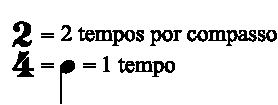
\includegraphics[scale=1]{formula-2tempos-por-compasso}
    }

    %%% PRÓXIMA LINHA
    \\
    \hline
    \letraquadrada{D}  &  \letraquadrada{E}  &  \letraquadrada{F}


    %%% PRÓXIMA LINHA
    \\
    \quadtitulo{Andamento}
    &
    \quadtitulo{Crescendo}
    &
    \quadtitulo{Decrescendo}

    %%% PRÓXIMA LINHA
    \\
    \textit{Andante}
    &
    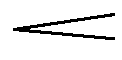
\includegraphics[scale=1]{crescendo}
    &
    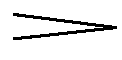
\includegraphics[scale=1]{decrescendo}

    \\
  \end{tabular}


  %%% PRÓXIMA TABELA
  \begin{tabular}[t]{|llll|}

    %%% PRÓXIMA LINHA
    \hline
    \multicolumn{4}{|l|}{\letraquadrada{G}}
    
    %%% PRÓXIMA LINHA
    \\
    \multicolumn{4}{|l|}{\quadtitulo{Acordes}}

    %%% CAVAQUINHO %%%%%%%%%%%%%%%%%%%%%
    %%% PRÓXIMA LINHA
    \\
    \multicolumn{4}{|l|}{\quadtitulo{Cavaquinho}}
    
    %%% PRÓXIMA LINHA
    \\
    \begin[fragment]{lilypond}
      \transpose c c { 
        \keepWithTag #'cv
        \include "acorde-D.ly"
      }
    \end{lilypond}
    &
    \begin[fragment]{lilypond}
      \transpose c c { 
        \keepWithTag #'cv
        \include "acorde-D7.ly" 
      }
    \end{lilypond}
    &
    \begin[fragment]{lilypond}
      \transpose c c {
        \keepWithTag #'cv
        \include "acorde-Am.ly"
      }
    \end{lilypond}
    &
    \begin[fragment]{lilypond}
      \transpose c c {
        \keepWithTag #'cv
        \include "acorde-E7.ly"
      }
    \end{lilypond}

    %%% BANDOLIM %%%%%%%%%%%%%%%%%%%%%
    %%% PRÓXIMA LINHA
    \\
    \hline
    \multicolumn{4}{|l|}{\quadtitulo{Bandolim}}
    
    %%% PRÓXIMA LINHA
    \\
    \begin[fragment]{lilypond}
      \transpose c c { 
        \keepWithTag #'bd
        \include "acorde-D.ly"
      }
    \end{lilypond}
    &
    \begin[fragment]{lilypond}
      \transpose c c { 
        \keepWithTag #'bd
        \include "acorde-D7.ly" 
      }
    \end{lilypond}
    &
    \begin[fragment]{lilypond}
      \transpose c c {
        \keepWithTag #'bd
        \include "acorde-Am.ly"
      }
    \end{lilypond}
    &
    \begin[fragment]{lilypond}
      \transpose c c {
        \keepWithTag #'bd
        \include "acorde-E7.ly"
      }
    \end{lilypond}


    %%% VIOLA %%%%%%%%%%%%%%%%%%%%%
    %%% PRÓXIMA LINHA
    \\
    \hline
    \multicolumn{4}{|l|}{\quadtitulo{Viola}}
    
    %%% PRÓXIMA LINHA
    \\
    \begin[fragment]{lilypond}
      \transpose c c { 
        \keepWithTag #'va
        \include "acorde-D.ly"
      }
    \end{lilypond}
    &
    \begin[fragment]{lilypond}
      \transpose c c { 
        \keepWithTag #'va
        \include "acorde-D7.ly" 
      }
    \end{lilypond}
    &
    \begin[fragment]{lilypond}
      \transpose c c {
        \keepWithTag #'va
        \include "acorde-Am.ly"
      }
    \end{lilypond}
    &
    \begin[fragment]{lilypond}
      \transpose c c {
        \keepWithTag #'va
        \include "acorde-E7.ly"
      }
    \end{lilypond}

    \\
    \hline
  \end{tabular}
\end{table}

%%%%%%%%%%%%%% CONTINUAÇÃO DA TABELA
\begin{table}[!ht]
  \centering
  \begin{tabular}[t]{|llll|}
    \hline

    %%% PRÓXIMA LINHA
    \multicolumn{4}{|l|}{\letraquadrada{G}}
    
    %%% PRÓXIMA LINHA
    \\
    \multicolumn{4}{|l|}{\quadtitulo{Acordes}}

    %%% VIOLÃO TENOR %%%%%%%%%%%%%%%%%%%%%
    %%% PRÓXIMA LINHA
    \\
    \multicolumn{4}{|l|}{\quadtitulo{Violão Tenor}}
    
    %%% PRÓXIMA LINHA
    \\
    \begin[fragment]{lilypond}
      \transpose c c { 
        \keepWithTag #'vt
        \include "acorde-D.ly"
      }
    \end{lilypond}
    &
    \begin[fragment]{lilypond}
      \transpose c c { 
        \keepWithTag #'vt
        \include "acorde-D7.ly" 
      }
    \end{lilypond}
    &
    \begin[fragment]{lilypond}
      \transpose c c {
        \keepWithTag #'vt
        \include "acorde-Am.ly"
      }
    \end{lilypond}
    &
    \begin[fragment]{lilypond}
      \transpose c c {
        \keepWithTag #'vt
        \include "acorde-E7.ly"
      }
    \end{lilypond}

    %%% VIOLÃO %%%%%%%%%%%%%%%%%%%%%
    %%% PRÓXIMA LINHA
    \\
    \hline
    \multicolumn{4}{|l|}{\quadtitulo{Violão}}
    
    %%% PRÓXIMA LINHA
    \\
    \begin[fragment]{lilypond}
      \transpose c c { 
        \keepWithTag #'vi
        \include "acorde-D.ly"
      }
    \end{lilypond}
    &
    \begin[fragment]{lilypond}
      \transpose c c { 
        \keepWithTag #'vi
        \include "acorde-D7.ly" 
      }
    \end{lilypond}
    &
    \begin[fragment]{lilypond}
      \transpose c c {
        \keepWithTag #'vi
        \include "acorde-Am.ly"
      }
    \end{lilypond}
    &
    \begin[fragment]{lilypond}
      \transpose c c {
        \keepWithTag #'vi
        \include "acorde-E7.ly"
      }
    \end{lilypond}

    %%% BAIXO %%%%%%%%%%%%%%%%%%%%%
    %%% PRÓXIMA LINHA
    \\
    \hline
    \multicolumn{4}{|l|}{\quadtitulo{Baixo}}
    
    %%% PRÓXIMA LINHA
    \\
    \begin[fragment]{lilypond}
      \transpose c c { 
        \keepWithTag #'bx
        \include "acorde-D.ly"
      }
    \end{lilypond}
    &
    \begin[fragment]{lilypond}
      \transpose c c { 
        \keepWithTag #'bx
        \include "acorde-D7.ly" 
      }
    \end{lilypond}
    &
    \begin[fragment]{lilypond}
      \transpose c c {
        \keepWithTag #'bx
        \include "acorde-Am.ly"
      }
    \end{lilypond}
    &
    \begin[fragment]{lilypond}
      \transpose c c {
        \keepWithTag #'bx
        \include "acorde-E7.ly"
      }
    \end{lilypond}


    %%% FINAL DAS LINHAS
    \\
    \hline
  \end{tabular}
\end{table}    

%%%%%%%%%%%%%%%%%%%%%%%% FINAL QUADRO 05 - VOL 1 %%%%%%%%%%%%%%%%%%%%%%%%%%%%%%%%













